\documentclass{book}
\title{Reti Logiche made Friendly}
\author{Matteo Sabella 218614}
\usepackage{graphicx}
\usepackage{wrapfig}
\usepackage[export]{adjustbox}
\usepackage{titlesec}
\usepackage{listings}
\usepackage{xcolor}
\usepackage{colortbl}
\graphicspath{{images/}}
\usepackage{wrapfig}
\definecolor{backcolour}{rgb}{0.95,0.95,0.92}
\definecolor{codegreen}{rgb}{0.4, 0.521, 0.454}
\definecolor{codegray}{rgb}{0.5,0.5,0.5}
\definecolor{codepurple}{rgb}{0.850, 0.203, 0.419}



\lstdefinestyle{mystyle}{
    backgroundcolor=\color{backcolour},   
    commentstyle=\color{codegreen},
    keywordstyle=\color{codepurple},
    numberstyle=\tiny\color{codegray},
    stringstyle=\color{codepurple},
    basicstyle=\ttfamily\footnotesize,
    breakatwhitespace=false,         
    breaklines=true,                 
    captionpos=b,                    
    keepspaces=true,                 
    numbers=left,                    
    numbersep=5pt,                  
    showspaces=false,                
    showstringspaces=false,
    showtabs=false,                  
    tabsize=2
}

\lstset{style=mystyle}





\begin{document}

\maketitle

Al mio fedele compagno di avventure, che mi piaceva girare a letto come un flip flop e che mi ha consentito di mantenere la fede.

\chapter{Da analogico a digitale}
Nell'era pre digitale i segnali erano analogici, ossia il loro valore spaziava su una gamma potenzialmente infinita di valori.
Ciò poneva di fronte ad un problema, quello delle interferenze e dei disturbi di segnale, che potevano distorcere o rendere impossibile la lettura del messaggio trasportato dal segnale in questione.
Si è perciò deciso di ricorrere al mezzo digitale, ossia un particolare modo di rappresentare le informazioni.
Ogni segnale può assumere solo due possibili valori( da qui denominato segnale binario), che si distinguono grazie ad un confine detto soglia che li separa.
Al di sotto di tale soglia il segnale ha ovunque lo stesso valore, così come al di sopra, ma tra una parte della soglia e l'altra, lì il valore cambia.
Tanto più il segnale è lontano dalla soglia tanto più esso può subire distorsioni senza che il messaggio venga all'arrivo compromesso.\\
Tale sistema però pone uno svantaggio, ossia l' impossibilità di comunicare un vasto numero di messaggi.
Per risolvere questo inconveniente intrinseco di questo modo di comunicare si ricorre a più sorgenti di segnali, così che invece che avere solo 2 possibili valori, il messaggio costituito da n segnali avrà \(2^n\) possibili significati o sfumature.\newline
\vspace{\baselineskip}
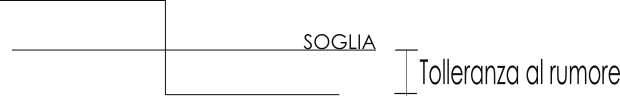
\includegraphics[width=\textwidth]{SchemaDigitale}
\chapter{Circuiti combinatori}
\section{Operatori}
\subsection{OPERATORI SEMPLICI}
Gli operatori basilari che vengono utilizzati per la costruzione di reti logiche sono i seguenti:\newline
\subsubsection*{AND}
\begin{wrapfigure}{r}{0.10\textwidth}
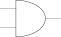
\includegraphics{AndPrecisa}
\end{wrapfigure}
L'operatore AND prende in input  due segnali e restituisce 1 se e solo se entrambi sono 1, altrimenti restituisce 0.
\newline Si rappresenta come : \(x*y\)\newline


\subsubsection*{OR}
\begin{wrapfigure}{r}{0.10\textwidth}
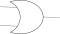
\includegraphics{OrGate}
\end{wrapfigure}
L'operatore OR prende in input due segnali e restituisce 1 se almeno uno dei due è 1, altrimenti restituisce 0.
\newline Si rappresenta come : \(x+y\)\newline
\subsubsection*{NOT}
\begin{wrapfigure}{r}{0.10\textwidth}
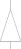
\includegraphics{NotGate}
\end{wrapfigure}
L'operatore NOT prende in input un solo segnali e restituisce 1 se il segnale è 0 e 0 se l'input è 1.
\newline Si rappresenta come : \(x'\)

\newpage
\subsection{OPERATORI COMPLESSI}
Gli operatori che vediamo di seguito possono essere considerati come operatori "complessi" ossia costituiti da elementi più semplici.
\begin{wrapfigure}{r}{0.10\textwidth}
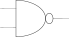
\includegraphics{NandGate}
\end{wrapfigure}
\subsubsection*{NAND}

L'operatore NAND è costituito da un operatore AND seguito da un NOT.
\begin{wrapfigure}{r}{0,10\textwidth}
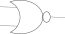
\includegraphics{NorGate}
\end{wrapfigure}
\subsubsection*{NOR}

L'operatore NOR è costituito da un operatore OR seguito da un NOT.

\subsubsection*{EXOR}
L'operatore EXOR è anche detto OR esclusivo, questo perchè restituisce 1 se e solo se i due segnali in ingresso sono diversi tra loro.
\subsubsection*{EXNOR}
L'operatore EXNOR è anche detto OR inclusivo perchè restituisce 1 se e solo se i due segnali in ingresso sono uguali tra loro.

\newpage
\section{Algebra di boole}
Le operazioni svolte dagli operatori appena visti godono di proprietà che vanno sotto il nome di algebra di Boole.\newline (Ognuna di esse è dimsotrabile tramite induzione completa, ossia verificando totalmente la veridicità delle implicazioni tramite tabelle di verità).
\subsection*{Identità}

\(x+0=x \) \newline
\(x*1=x \)

\subsection*{Proprietà commutativa}

\(x+y=y*x \) \newline
\(x*y=y*x \) 

\subsection*{Proprietà distributiva}

\( x*(y+z)=(x*y)+(x*z)  \) \newline
\( x+(y*z)=(x+y)*(x+z)  \)

\subsection*{Complementazione}

\(x+x'=1 \) \newline
\(x*x'=0 \)

\subsection*{Proprietà associativa}

\(x+(y+z)=(x+y)+z \) \newline
\(x*(y*z)=(x*y)*z \) 

\subsection*{Leggi di De Morgan}

Consentono di trasformare delle funzioni in cui compaiono OR in funzioni equivalenti che usano delle AND.

\( (x+y)' = x' * y' \) \hspace{3cm} \( (x'+y')' = x*y\) \newline
\( (x*y)' = x' + y' \) \hspace{3cm} \( (x'*y')'= x+y\)
\newline
Tip : un modo utile per ricordarsele è che per passare da un operatore ad un altro , si cambia l'operatore e si "raccoglie" un not.

\newpage
\section{Teorema Di Shennon}
Nel processo di ricerca di un'espressione logica che impieghi gli operatori che ora conosciamo, torna utilissimo il teorema di Shennon.
Per ogni funzione logica del tipo\break\newline \( f({x_1},{x_2},{x_3},...,{x_n}) \)\break\newline vale la seguente uguaglianza.\newline \(f({x_1},{x_2},{x_3},...,{x_n})=a*f(1,{x_2},{x_3},...,{x_n})+a'*f(0,{x_2},{x_3},...,{x_n})\)\break\newline
Questa uguaglianza è valida perchè se a valesse 1, allora la parte di destra dell'OR sarà un AND con sicuramente valore 0 e quindi verrà come risultato il valore della prima espressione, altrimenti se a fosse 0 varrebbe lo stesso discorso ma al contrario.
\paragraph*{}
Procedendo iterando questo teorema sui pezzi di funzioni rimanenti si può arrivare ad un'espansione nella seguente forma:


\(f({x_1},{x_2},{x_3},...,{x_n})=a*f(1,{x_2},{x_3},...,{x_n})+a'*f(0,{x_2},{x_3},...,{x_n})\)

\newpage

\chapter{Semplificazione di funzioni logiche}
Introduciamo ora alcune definizioni:\newline\break
\begin{itemize}
\item\textbf{Letterale}
Ogni variabile che sia affermata o negata.\\
\item\textbf{Minterm}
Prodotto in cui ogni variabile compare una volta come letterale.\newline Esso è 1 per una e una sola combinazione di letterali.\\
\item\textbf{Maxterm}
Somma in cui variabile compare una volta come letterale.\newline Esso è 0 per una e una sola combinazione dei suoi letterali.\\
\item\textbf{Implicante}
f è implicante di g se e solo se quando f è 1 allora g è 1.
\vspace{\baselineskip}
\newline Si dice \textbf{implicante primo} ogni implicante che non è possibile racchiudere in uno più grande.
Essi possono essere \textbf{ridondanti} nel caso in cui coprano zone coperte da altri implicanti primi mentre altri sono invece \textbf{essenziali} perchè sono gli unici a coprire quelle zone.

\vspace{\baselineskip}

Ogni minterm è un implicante della propria f, l'unico problema è che ognuno di essi rappresenta "pochi uni".\newline\break
\end{itemize}



\newpage

 La funzione logica sarà data dall' \text{OR} degli implicanti, ma quali cerco ?
\vspace{\baselineskip}

Partendo dalla tabella della verità si possono trovare i minterm della funzione.\\Questi poi possono essere compattati utilizzando le proprietà dell'algebra di Boole (torna molto utile l'adiacenza logica).

L'adiacenza logica in particolare si può utilizzare solo quando, dati minterm composti da L letterali, L-1 letterali restano immutati ed uno solo cambia.

Per trovare implicanti che non siano minterm è utile utilizzare la \textbf{notazione Gray}.\\
Chiamiamo \textbf{term} gli implicanti che non sono minterm !.\\
Essa consiste nel fare tabelle di verità in cui tra ogni riga e la sua successiva c'è solamente una variabile a variare, così da poter eventualmente fare dei raccoglimenti sfruttando l'algebra di Boole.


Non garantisce tuttavia un modo perfetto per trovare i minterm con facilità perchè permette di muoversi in una sola dimensione.

\vspace{\baselineskip}

Nel caso funzioni con più di due variabili è necessario cercare gli implicanti utilizzando altri modi per rappresentare le tabelle di verità così da far risaltare meglio le adiacenze tra i vari minterm.\\
\vspace{\baselineskip}
Qui entra in gioco \textbf{la mappa di Karnough}
\vspace{\baselineskip}
\begin{tabular}{|c|c|c|c|c|}
\hline
a\backslash bc & 00 & 01 & 11 & 10 \\
\hline
0              & *  & *  & *  & *  \\
\hline
1              & *  & *  & *  & *  \\
\hline
\end{tabular}
\vspace{\baselineskip}
Nella prima riga partendo dall'alto verranno messe in notazione Gray tutte le possibili combinazioni che la variabile bc può assumere.
Nella prima colonna invece tutte le combinazioni (in questo caso solo due) che la variabile a può assumere.

Nelle celle interne invece si procederà mettendo ad ogni incrocio, al posto di * l'uscita della funzione per i corrispondenti valori di a,b e c.


...


\newpage
\section{Insiemi di operatori completi ed uso delle porte logiche}

\section{Mappe a 4,5 e 6 variabili}
Le mappe saranno fatte esattamente come fatto fino a qui con la differenza che aumenterà la loro dimensione in modo esponenziale.
Infatti per ogni variabile che aggiungiamo le possibili combinazioni degli ingressi vengono raddoppiate !
(Continueremo ad usare il codice Gray)
Avremo quindi per mappe a 4 variabili delle mappe quadrate i cui minterm saranno composti da 4 letterali.

\section{Altri metodi per sintetizzare circuiti}
\section{Minimizzazione congiunta}
\newpage	
\chapter{Circuiti Combinatori Fondamentali}

Di seguito vengono rappresentati, analizzati e spiegati alcuni circuiti combinatori che sono ritenuti fondamentali in quanto compaiono molto spesso e per cui è bene ricordarsi come sono fatti per non perdere tempo.
\section{Multiplexer}
In generale un multiplexer è una funzione logica che tramite un criterio prende delle variabili in entrata e ne restituisce una di esse.
\subsection{Da 2 a 1}
Ora prendiamo in esame il più elementare tra i multiplexer, ovvero quello che fa una decisione tra due varibili in ingresso.
Questo è il più elementare perchè altrimenti avrei una variabiule in ingresso ed una in uscita e ciò non è un vera scelta.

Partiamo dalla tabella di verità scritta con il codice Gray e cerchiamone gli implicanti primi.
Partiamo da qui perchè è il punto principale per impostare come funzionerà il nostro multiplexer.\\

\begin{tabular}{|c|c|c|c|c|}
\hline
S-AB & 00 & 01 & 11 & 10 \\ \hline
0 &    0  &  0 & \cellcolor{yellow}1  & \cellcolor{yellow}1  \\ \hline  
1 &    0  &  \cellcolor{yellow}1 & \cellcolor{yellow}1  & 0  \\
\hline
\end{tabular}\break


Gli implicanti primi sono: SB, AB, S'A.
Quindi la nostra funzione può essere scritta come segue:
\( f=\) SB+S'A

Cerchiamo di capire cosa ci sta dicendo questa funzione.
Premettiamo che la convenzione che S=0 selezioni A mentre S=1 selezioni B è nostra scelta, con alcune differenze può avvenire benissimo anche il caso in cui S=0 selezioni B mentre S=1 selezioni A.

Prendendo in esame uno solo delle AND, queste ci dicono che nel caso in cui S sia 0 SICURAMENTE quel termine sarà del tutto irrilevante nel passaggio successivo costituito da un OR.
Perciò verrà selezionato ESCLUSIVAMENTE l'operazione AND che ha S=1.
Poi l'essere 0 o 1 dell'altro operando determinerà l'uscita esattamente di quel valore.



\begin{wrapfigure}{r}{0,1\textwidth}
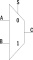
\includegraphics{Multiplexer21}
\end{wrapfigure}


Il multiplexer 2 a 1 si rappresenta con un questo simbolo circuitale:
In cui i numeri indicano per quale valore di S venga selezionata la corrispondente entrata.

\begin{figure}
\centering
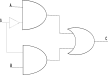
\includegraphics{Multiplexer21Circuito}
\caption{schema circuitale di un Multiplexer 2 a 1}
\end{figure}


\subsection{Da 4 a 1}

Alla luce di quello che abbiamo appena letto riguardo al multiplexer 2 a 1 possiamo immaginare come realizzare questa versione più in grande.

Posso utilizzare due multiplexer 2 a 1 per ottenere due output e poi questi ultimi metterli all'interno di un ulteriore multiplexer 2 a 1 così da ottenere un solo risultato in uscita.

\(S_01 \) si occuperà di scremare tra A e B mentre \(S_02 \) scremerà tra C e D.


\section{Odd Function}

E' una funzione che vale 1 SOLO se il numero di ingressi ad 1 è dispari.\\
Iniziamo sviluppando la tabella di Karnaugh.\\

\vspace{\baselineskip}

\begin{tabular}{|c|c|c|c|c|}
\hline
a\backslash bc & 00 & 01 & 11 & 10 \\
\hline
0              & 0  &  \cellcolor{yellow}1 & 0  & \cellcolor{yellow}1  \\
\hline
1              & \cellcolor{yellow}1  &  0 & \cellcolor{yellow}1  & 0  \\
\hline
\end{tabular}
\vspace{\baselineskip}

Purtroppo i term in questo caso coincidono con i minterm della tabella di karnaugh e sono : ab'c' , a'b'c , abc , a'bc.

Quindi la funzione logica dell' odd counter è :

\(f=\)ab'c'+a'b'c+abc+a'bc'

Possiamo ora procedere a raggruppare eventuali term sfruttando l'adiacenza logica.

\(f=\)b'(ac'+a'c)+b(ac+a'c') che possiamo ulteriormente compattare riconoscendo in ac'+a'c l'operatore booleano XOR e in ac+a'c l'operatore booleano XNOR.




\section{Conta Uni}

Lo scopo di questo circuito è dire in uscita quanti degli ingressi sono a 1. Nel nostro caso ci saranno 3 ingressi, quindi il numero in uscita potrà variare da 0 a 3 ossia da 00 a 11 in binario.


Chiamando gli ingressi a,b,c e le uscite s1 ed s2 , agiamo sulle uscite con due mappe di karnaugh distinte ma che in realtà sono parallele e sinergiche nel circuito.


Iniziamo con s1, che rappresenterà il bit meno significativo del risultato e perciò dovrà essere 1 nel caso in cui in ingresso ci siano 1 (01) o 3(11) "uni" in ingresso.

\vspace{\baselineskip}
\begin{tabular}{|c|c|c|c|c|}
\hline
a \backslash bc & 00 & 01 & 11 & 10 \\
\hline
0              & 0  & {\cellcolor{yellow} 1 } &  0 & {\cellcolor{yellow}1}  \\
\hline
1             & {\cellcolor{yellow}1}  & 0  &  {\cellcolor{yellow}1} & 0  \\
\hline
\end{tabular}
\newline \vspace{\baselineskip}
Per s2 l'operazione sarà la stessa con la differenza che l'uscita sarà ad 1 nei casi in cui la quantità di "uni" in ingresso sia 2 (10) o 3 (11).
\newline\vspace{\baselineskip}
\begin{tabular}{|c|c|c|c|c|}
\hline
a\backslash bc & 00 & 01 & 11 & 10 \\
\hline
0              & 0  & 0  &  \cellcolor{yellow}1 & 0  \\
\hline
1              & 0  & \cellcolor{yellow}1  &  \cellcolor{yellow}1 & \cellcolor{yellow}1  \\
\hline
\end{tabular}




Possiamo perciò ricavare le funzioni logiche per l'uscita s1 ed s2.

\begin{itemize}
\item{S1} \\ Osservando la mappa di Karnaugh si può riconoscere nella funzione s1 la stessa forma che poco fa abbiamo chiamato odd function, infatti è proprio quella la funzione di questa uscita.

Perciò \(f_{S1}=\)ab'c'+a'b'c+abc+a'bc'

\item{S2} \\ Qui invece richiede la ricerca da parte nostra di term all'interno della mappa, da cui otteniamo la seguente funzione : \(f_{s2}=\)bc+ac+ab .

\section{Codifica e decodifica}

\subsection{Priority Encoder}

Il priority encoder è un circuito la cui uscita corrisponderà all'indice dell'input con maggior precedenza ad 1. 
Quindi prima di tutto è necessario assegnare ad ogni ingresso un indice, ossia un valore che lo identifichi.
Nel nostro caso avremmo tre ingressi : a,b,c e perciò una possibile corrispondenza per gli indici è l'uso dei numeri 1,2,3 rispettivamente. Per nostra scelta imponiamo che a(ossia 1) sia quello con priorità minore, mentre c(ossia 3 ) quello con priorità maggiore.

(Gli indici saranno smostrati in formato binario e perciò dato che abbiamo solo 3 ingressi basteranno 2 uscite perchè saranno da mostrare solo i valori 00, 01,10,11).

Procediamo quindi con la tabella della verità:

\begin{tabular}{|c|c|c|c|c|}
a(1) & b(2) & c(3) & s1 & s2 \\
\hline
0 & 0 & 0 & 0 & 0 \\
\hline
0 & 0 & 1 & 1 & 1 \\
\hline
0 & 1 & 1 & 1 & 1 \\
\hline
1 & 1 & 1 & 1 & 1 \\
\hline
1 & 0 & 1 & 1 & 1 \\
\hline
0 & 1 & 0 & 1 & 0 \\
\hline
1 & 1 & 0 & 1 & 0 \\
\hline
1 & 0 & 0 & 0 & 1 \\
\hline

\end{tabular}

Passiamo ora alle mappe di Karnaugh.

S2, che rispecchierà la cifra meno significativa del risultato, avrà la seguente tabella:

\begin{tabular}{|c|c|c|c|c|}
a\backslash bc & 00 & 01 & 11 & 10 \\
\hline
0              & 0  & \cellcolor{yellow}1  &  \cellcolor{yellow}1 & 0  \\
\hline
1              & \cellcolor{yellow}1  & \cellcolor{yellow}1  &  \cellcolor{yellow}1 & 0  \\
\hline

\end{tabular}

S1 invece che rispecchierà la cifra più significativa del risultato sarà:

\begin{tabular}{|c|c|c|c|c|}
a\backslash bc & 00 & 01 & 11 & 10 \\
\hline
0              & 0  & \cellcolor{yellow}1  &  \cellcolor{yellow}1 & \cellcolor{yellow}1  \\
\hline
1              & 0  & \cellcolor{yellow}1  &  \cellcolor{yellow}1 & \cellcolor{yellow}1  \\
\hline

\end{tabular}


Perciò le equazioni che rispecchiano le uscite sono :

\(f_{s1}=\)c+b \\
\(f_{s2}=\)c+ab'


E il circuito rappresentante il priority encoder è il seguente:


\section{Indifferenze o don't care}

\chapter{Tempistiche e diagrammi temporali}

In un circuito ci sono dei ritardi tra quanto il segnale entra in una porta e quando ne esce il risultato prodotto dalla logica della porta stessa.
Questi ritardi sono dati da motivi fisici e di solito sono specificati al momento dell'acquisto della porta così da permettere di scegliere quella più adatta agli scopi per cui verrà impiegata.

I diagrammi temporali sono di due tipi:
 
\textbf{SENZA RITARDO}\newline
Quelli senza ritardi vengono impiegati per valutare la funzione logica ed effettuare operazioni di debugging se necessarie.\newline
\textbf{CON RITARDO}\newline
Quelli con ritardi invece vengono utilizzati per valutare le prestazioni della funzione logica.\newline

Un tempo utile da conoscere riguardo ad un circuito logico è quello massimo che può impiegare per restituire una risposta all'input sottopostogli.


\section{Ottenere il diagramma temporale di un circuito}

Prima di tutto è necessario identificare i nodi interni e assegnargli un nome identificativo.

Poi si procede identificando gli stimoli di ingresso e successivamente si valuta l'uscita di ogni nodo sulla base degli ingressi che ha ricevuto.



\section{Glitch}

In un circuito possono verificarsi dei fenomeni detti \textbf{Alee o Glitch} e sono dovuti a brevi e rapidi cambiamenti di valore che avvengono con particolati combinazioni di ritardi. Influiscono sul risultato istantaneo ottenibile dal circuito (transitorio) ma non sulla correttezza della funzione logica.


Per ovviare a ciò si utilizza la tipologia di\textbf{ circuito sincrono}

\subsection{Alee su Karnaugh}

\chapter{Circuiti aritmetici}

Si chiamano \textbf{circuiti aritmetici} tutti quei circuiti che sfruttano porte logiche e il sistema di numerazione binario per effettuare operazioni di calcolo.


\section{Struttura iterativa generica}

Siccome il numero degli ingressi cresce con il numero delle cifre ben presto le dimensioni di input diventano ingestibili ecco che quindi si può ricorrere ad un metodo gerarchico, ossia un metodo iterativo che sfrutta un'operazione atomica e la replicaquante volte è necessario.


\section{Somma}

\subsection{Half adder}
Iniziamo con la tabella di verità del circuito che dovrebbe sommare due ingressi da 1 bit ciascuno.
Esso restituirà un risultato con 2 bit in uscita.
Indichiamo con a e b i due ingressi, mentre con s il bit meno significativo del risultato e con c quello più significativo.
La lettera c ci ricorderà anche che tale cifra è dovuta al carry dell'operazione.
\newline
\begin{tabular}{|c|c|c|c|}

\hline
a & b & c & s \\ \hline
0 & 0 & 0 & 0 \\ \hline
0 & 1 & 0 & 1 \\ \hline
1 & 1 & 1 & 0 \\ \hline
1 & 0 & 0 & 1 \\ 
\hline
\end{tabular}



Mettendo s e c in due mappe di Karnaugh separate si possono costruire le funzioni logiche di ognuno.\\
Iniziamo con S:

\begin{tabular}{|c|c|c|}
\hline
a/b & 0 & 1 \\ \hline
0   & 0 & \cellcolor{yellow}1 \\ \hline
1   & \cellcolor{yellow}1 & 0 \\ \hline
\end{tabular}

La funzione logica che rappresenta l'uscita s quindi è \(f_s=\)aXORb .\\
Passando a C otteniamo poi:

\begin{tabular}{|c|c|c|}
\hline
a/b & 0 & 1 \\ \hline
0   & 0 & 0 \\ \hline
1   & 0 & \cellcolor{yellow}1 \\ \hline
\end{tabular}

La funzione logica che esprime il comportamento di C è \(f_c=\)aANDb .

Il circuito dell'half adder è:


\subsection{Full adder}

L'half adder però non tiene conto di un'evetuale riporto proveniente dal calcolo fatto in precedenza.
Infatti se vogliamo sfruttare un'architettura gerarchica bisogna tener conto che la somma atomica fatta per la cifra con un grado di significatività in meno rispetto a quella che stiamo sommando potrebbe aver generato un carry con la conseguente necessità di doverne tener conto ora che facciamo la somma.


Il problema si risolve aggiungendo un ingresso all'half adder per poter tenere conto di un0 eventuale carry non nullo.

\begin{tabular}{|c|c|c|c|c|}
\hline
a & b & c & C & s \\
\hline
0 & 0 & 0 & 0 & 0 \\
\hline
0 & 0 & 1 & 0 & 1 \\
\hline
0 & 1 & 1 & 1 & 0 \\
\hline
1 & 1 & 1 & 1 & 1 \\
\hline
1 & 1 & 0 & 1 & 0 \\
\hline
1 & 0 & 0 & 0 & 1 \\
\hline
1 & 0 & 1 & 1 & 0 \\
\hline
0 & 1 & 0 & 0 & 1 \\
\hline 

\end{tabular}



La mappa di Karnaugh per il valore di S è :

\begin{tabular}{|c|c|c|c|c|}
\hline
c\backslash ab & 00 & 01 & 11 & 10 \\
\hline
0              & 0  & \cellcolor{yellow}1  &  0 & \cellcolor{yellow}1  \\
\hline
1              & \cellcolor{yellow}1  & 0  & \cellcolor{yellow}1  & 0  \\
\hline
\end{tabular}

La mappa di Karnaugh per il valore di C è :

\begin{tabular}{|c|c|c|c|c|}
\hline
c\backslash ab & 00 & 01 & 11 & 10 \\
\hline
0              & 0  & 0  &  \cellcolor{yellow}1 & 0  \\
\hline
1              & 0  & \cellcolor{yellow}1  & \cellcolor{yellow}1  & \cellcolor{yellow}1  \\
\hline
\end{tabular}

COnfrontando il circuito con quelli che abbiamo già visto ci si accorge che è lo stesso circuito del conta uni !

\subsection{Sommatore ripple carry}
Ora quindi possiamo unire i circuiti dell'half adder e del full adder per ottenere un sommatore con un arbitrario numero di ingressi.
Analogamente possiamo ottenere un sommatore con arbitrario numero di ingressi anche con tutti e soli full adder a patto però di mettere a 0 l'adder della cifra meno significativa così da renderlo un half adder a tutti gli effetti.

Il numero di uscite del ripple carry è pari al numero di ingressi +1 perchè deve anche mostrare un eventuale riporto dovuto all'ultimo sommatore.


\subsubsection*{Prestazioni}

Il sommatore ripple carry ha dimensioni ridotte che aumentano linearmente con l'aggiunta di degli ingressi.

La catena dei carry forma un cammino molto lungo e ciò fa si che il sommatore sia lento con una lentezza proporzionale al numero di bit .

Ciò fa si che sussistano delle alee impossibili da eliminare che fanno cambiare il risultato finchè il carry non si è propagato fino all'ultimo full adder.
Questo perchè gli adder calcolano la somma prima che un eventuale carry venga comunicato dagli adder che si occupano delle cifre meno significative e quindi in caso di carry non nullo dovrà rifare il calcolo per quella cifra.


\subsection{Sommatore carry look-ahead}

Permette di ottimizzare il calcolo del carry riducendo a 2 livelli questa operazione. Ciò a però complica la realizzazione.

Si comincia separando la somma dal carry. 


\section{Sottrazione}

Molto siile alla somma però ora ci possono essere dei prestiti dalle cifre più significative.
Inoltre il risultato può essere negativo.


Nel caso di risultati negativi, il calcolo si fa scambiando i numeri e poi mettendo un bit di segno.

Scambiare però i numeri è come scambiare due cavi, è un'operazione complicata !

Molto più semplice è l'uso di \textbf{notazione in complemento a 2}. 

\subsection{Notazione in complemento a 2}

La notazione in complemento a 2 permette di rappresentare i numeri negativi in binario in un modo che a noi torna comodo per poterci fare operazioni algebriche.\\
Solitamente con n bit a disposizione noi avremmo la possibilità di rappresentare \(2^n\) numeri in binario, che sono i numeri da 0 (n zeri) fino a \(2^n-1\) (n uni).

Con la notazione in complemento a 2 invece un qualsiasi numero M è rappresentato come \(2^n-M\).

\begin{itemize}
\item{\(M<2^n\)}
Per esempio avendo 3 bit [*][*][*] e volendo rappresentare il numero 5 in binario si avrebbe [1][0][1].
In complemento a 2 questo è [1][1][1]-[1][0][1]=[0][1][0] ossia 2.
\item{\(M>2^n\)}
Per esempio avendo 3 bit [*][*][*] e volendo rappresentare il numero -3 in binario in complemento a 2 , [1][1][1]+[0][1][1]= [1][0][1][0] ossia 9.

\end{itemize}

Questo perchè mettendo in una tabella il complemento a 2 si ottiene il seguente risultato:

\begin{tabular}{|c|c|c|c||c|c|c|c|}
\hline
4 & 2 & 1 & M & -4 & 2 & 1 & M  \\
\hline
0 & 0 & 0 & 0 &  0 & 0 & 0 & 0  \\
\hline
1 & 1 & 1 & 7 &  1 & 1 & 1 & -1 \\
\hline
1 & 1 & 0 & 6 &  1 & 1 & 0 & -2 \\
\hline
1 & 0 & 1 & 5 &  1 & 0 & 1 & -3 \\
\hline
1 & 0 & 0 & 4 &  1 & 0 & 0 & -4 \\
\hline
0 & 1 & 1 & 3 &  0 & 1 & 1 & 3  \\
\hline
0 & 1 & 0 & 2 &  0 & 1 & 0 & 2  \\
\hline
0 & 0 & 1 & 1 &  0 & 0 & 1 & 1  \\
\hline
\end{tabular}





\newpage
\section{Moltiplicazione}

Volendo moltiplicare due numeri POSITIVI si può ancora una volta sfruttare la struttura gerarchica.

Utilizzando la rappresentazione binaria le moltiplicazioni tra due numeri possono essere costituite dalle seguenti combinazioni :

\begin{tabular}{|c|c|c|}
\hline
a & b & res \\
\hline
0 & 0 & 0 \\
\hline
1 & 0 & 0 \\
\hline
0 & 1 & 0 \\
\hline
1 & 1 & 1 \\
\hline
\end{tabular}

Quello sopra descritto è esattamente il comportamento della porta AND, per convincersene basta confrontare le due tabelle della verità.


Perciò il prodotto di due numeri ciascuno costituito da 1 bit ha come risultato l'operazione logica AND tra di essi.

Rendiamo ora il moltiplicatore multi-bit tramite struttura gerarchica:

Dati due numeri a e b rispettivamente con m e n bit ciascuno, il moltiplicatore a*b sarà una concatenazione in cui il bit meno significativo di b moltiplicherà tutto a e questo si fa mettendo m porte and in cui entrano una cifra di a e la meno significativa di b.
Poi ciò produce un risultato, il cui bit meno significativo sarà il bit meno significativo del risultato finale mentre invece il resto del risultato è parziale e dovrà essere sommato al risultato della moltiplicazione tra le cifre di a e il bit secondo bit meno significativo.
Iterando questo processo si ottiene il risultato cercato.

Attenzione che mentre la somma tra due numeri con n cifre può produrre al massimo un numero con n cifre+1 il prodotto tra due numeri di m ed n cifre può produrre un numero di cifre fino a 2*n, in quanto ogni moltiplicazione produce n cifre e per ogni risultato parziale ci sarò uno shift verso sinistra di 1 quindi alle n cifre si sommano n-1 cifre +1 per un eventuale carry out .

Il circuito del moltiplicatore multi-bit è il seguente :


\chapter{Linguaggi di descrizione dell'hardware}

Una volta progettato un circuito e disegnato si potrebbe procedere a comprare le porte logiche ed assemblarlo ma la natura di test che quindi impone un alto tasso di variabilità del circuito durante la fase di progettazione ed affinamento e la crescente dimensione dei circuiti al giorno d'oggi non favoriscono questo approccio.
Molto meglio è invece utilizzare un linguaggio di descrizione che permette di simulare il funzionamento delle porte e quindi dei circuiti.


\section{Programmi richiesti: ghdl e gtkwave}

I programmi che andremo ad utilizzare sono ghdl e gtkwave.\\
Una volta scaricate le versioni stabili correnti adatte al vostro dispositivo si consiglia di estrarre i contenuti di entrambe le cartelle in due cartelle separate.\\
Poi aggiungere nel caso di windows i percorsi delle cartelle bin al PATH così da poterci accedere ogni volta senza dover andare nel percorso preciso in cui andremo a mettere gli eseguibili.

\subsubsection*{ghdl}
\subsubsection*{gtkwave}
\subsubsection*{Comandi frequenti}

I comandi più frequenti sono:

\begin{verbatim}ghdl -h \end{verbatim}visualizzo i comandi che ghdl offre.

\begin{verbatim}
-a nomedelfile
\end{verbatim}
Compila il file .vhd che gli indichiamo
\begin{verbatim}
-e UNIT
\end{verbatim}
E' un passaggio necessario ai fini dell'esecuzione. Nel token UNIT va specificato il nome della entity che poi abbiamo intenzione di eseguire.
\begin{verbatim}
-r UNIT
\end{verbatim}

Questo comando esegue l'architettura dell'entità che inseriremo al posto di UNIT e che prima dovrà essere passata per i comandi -a e -e.
\end{verbatim}


Quindi se volessimo compilare ed eseguire l'entità baseEntity nel file baseTest.vhd seguiremo i seguenti passaggi:
\begin{verbatim}
ghdl -a baseTest.vhd
ghdl -e baseEntity
ghdl -r baseEntity
\end{verbatim}

\section*{VHDL}

Il linguaggio che utilizzeremo è il \textbf{VHDL}, ossia \textbf{V}ery highspeed integrated circuit \textbf{H}ardware \textbf{D}escription \textbf{L}anguage.

Il VHDL ci permette di lavorare secondo 3 \textbf{metodologie}

\begin{itemize}
\item \textbf{Top-Down}
\item \textbf{Buttom-Up}
\item \textbf{Meet In The Middle}
\end{itemize}

e secondo 3 viste

\begin{itemize}
\item \textbf{Data flow}: \newline Consiste nella descrizione delle uscite in funzione degli ingressi. E' specificata con equazioni booleane messe a sistema tra loro.
\item \textbf{Strutturale}:\newline Consiste nella descrizione del circuito grazie all'utilizzo di componenti già esistenti che verranno combinati ed aggregati tra di loro. 
\item \textbf{Comportamentale}: \newline Consiste nella descrizione del circuito tramite l'algoritmo che dovrà implementare.
\end{itemize}


\newpage
\subsection{Entità}

La nozione di \textbf{entità} in VHDL corrisponde alla rappresentazione di un blocco \textbf{SENZA SPECIFICARNE} la logica interna ma solamente l'interfaccia con l'esterno.

Esso specifica :
\begin{itemize}
\item \textbf{nome}
\item \textbf{numero di ingressi}
\item \textbf{numero di uscite}

\end{itemize}

Di seguito il codice per dichiarare un'entità di nome "name\textunderscore entity" con n ingressi e m-n uscite.

\begin{lstlisting}[language=VHDL]
entity nome_entity is
port
(	
	nome_porta1 : tipo_ingresso,
	nome porta2 : tipo_ingresso,...
	nome_portan : tipo_ingresso;
	nome_portan+1 : tipo_uscita,
	nome_portan+2 : tipo_uscita,...
	nome_portan+3 : tipo_uscita;
);
end entity nome_entity;
\end{lstlisting}

\subsection{Architettura}

La nozione di \textbf{architettura} in VHDL specifica il comportamento di un'entità.
(Ad un'entità possono corrispondere più architetture.)

\begin{lstlisting}[language=VHDL]

architecture nome_architettura of nome_entita is
--dichiarazione di eventuali signal o buffer ausiliari
begin
--le equazioni e le operazioni di assegnamento che verranno scirtte in questa zona verranno eseguite tutte in contemporanea, indipendentemente dalla sequenza in cui compariranno


end architecture nome_architettura;


\end{lstlisting}

ATTENZIONE ! a differenza di linguaggi come il C, in VHDL l'operatore di assegnazione è '<=' mentre quello di comparazione di uguaglianza è '='.

Per l'assegnazione si scrive a<=b per indicare che il valore di b viene assegnato ad a.

\subsection{Testbench}

Il \textbf{testbench} è un'unione della vista dataflow con quella strutturale che permette la simulazione del circuito dando dei dati in ingresso.

\begin{lstlisting}[language=VHDL]

--dichiaro un entita senza interfaccia perche non ha necessita di porte di ingresso ne di uscita.
entity TestBench is 
end entity TestBench;

--definisco ora la sua architettura

architecture test of TestBench is 

--segnali interni di interconnessione
signal a,b,c : bit;

begin
--istanzio il modulo da testare
g1 : entitadatestare port map()

--definizione degli stimoli tramite equazioni in cui assegno ogni tot secondi un certo valore ai signal del mio testBench che a loro volta verranno assegnati alle porte dell entita da testare.

\end{lstlisting}

Il testbench può essere fatto nello stesso file di testo in cui si dichiarano le entità e le architetture che poi andranno ad essere usate.


\subsection*{Components}

Può capitare di avere una funzione logica implementata in un file e di volerla recuperare all'interno di un progetto più ampio o per eseguirne un test bench ma senza sporcare il codice.

Per fare ciò è necessario dunque all'interno del nuovo file pescare questa risorsa e ciò è possibile tramite un component.


\begin{lstlisting}[language=VHDL]
component nomecomponent is 

--descrizione dell' entita

end component;
\end{lstlisting}


\section*{Operatori,Identificatori e operazioni multiple}

Il linguaggio VHDL ha di default tutti gli operatori booleani .
L'operatore \textbf{NOT} è l'unico con la \textbf{priorità alta} mentre gli altri hanno tutti la stessa priorità e quindi verrà data importanza all'ordine o ad eventuali parentesi per decidere quale operazione fare per prima.\newline
VHDL è un linguaggio NON case sensitive.

Per specificare un delay si può utilizzare l'operatore \textbf{after}
Con il tipo bit\_vector(n down to m) si crea un array di bit con gli indici che vanno da m ad n.
VHDL possiede tutte le operazioni booleane come and,or,xor.
\break \nextline
La precedenza maggiore tra tali operazioni la ha la porta NOT mentre a differenza di quello che avviene nell'algebra booleana il resto degli operatori ha la stessa priorità perciò per forzare alcune operazioni prima di altre bisogna usare le parentesi !\nextline
Nella descrizione delle architetture a volte è necessario instanziare variabili interne, queste vengono chiamate \textbf{signal} e necessitano di un nome univoco per essere riconosciuti nello svolgimento della logica del componente.\break\nextline
(Attenzione che VDHL NON è case sensitive).

\section*{Parametri formali ed effettivi}

Le funzioni si richiamano nell'architettura tramite \textbf{port map} seguito da \textbf{notazione posizionale} e la loro instanziazione sarà contemporanea.
All'interno della stessa architettura possono avvenire \textxtbf{più operazioni}. L'ordine in cui vengono specificate all'interno dell'architettura non è rilevante perchè vanno concepite come un sistema in cui \textbf{procedono in parallelo}.

\begin{lstlisting}[language=VHDL]
nome_istanza : nome_master port map(parametri effettivi)
\end{lstlisting}
Si può anche optare per un'assegnazione di tipo esplicito e ciò aiuta a devitare gli errori e ad indentificarli prima.

\newpage
\section{Modi dei segnali}

I segnali possono assumere vari tipologie e ognuna di esse comporta un certo set di operazioni ammesse o no.

\begin{itemize}

\item\textbf{IN}
I segnali in in possono essere solamente letti e perciò possono stare solo a destra dell'operatore di assegnazione.

\item\textbf{OUT}
I segnali di out possono essere solo scritti e perciò staranno solamente dalla parte dell'operatore di assegnazione che subisce l'assegnamento.
Inoltre nelle quazioni all'interno di un'architettura possono comparire una volta sola, questo perchè none ssendo sequenziali bensì contemporanee le istruzioni avrei un conflitto nell'assegnazione.

\item\textbf{BUFFER}
I segnali buffer sono segnali in out ma leggibili e perciò possono stare da entrambe le parti di un'assegnazione.
Ma possono subire un'assegnazione comunque una sola volta.

\begin{lstlisting}[language=VHDL]
port(var : buffer bit);
\end{lstlisting}

\item\textbf{SIGNAL}
Sono segnali sia in ingresso sia in uscita ( venendo valutati una volta sola).

\begin{lstlisting}[language=VHDL]
--si scrive nell'architecture PRIMA del begin
signal S: bit_vector(3 downto 1);
\end{lstlisting}

\item\textbf{INOUT}
Sono componenti analoghi ad i buffer ma possono avere driver dall'esterno.

Possono subire assegnazioni più volte ma stando attenti ai conflitti. (es. buffer tri-state)

\begin{lstlisting}[language=VHDL]
--in entity
port (bus: inout bit)
\end{lstlisting}
\item\textbf{GENERIC}

Permette di parametrizzare un segnale così da rendere un'entità più versatile e riutilizzabile.

nella definizione dell'entità si scrive
\begin{lstlisting}[language=VHDL]
generic(nomesegnale : tiposegnale)
\end{lstlisting}

poi nella definizione dell'architettura di quella data entità si scriverà 
\begin{lstlisting}[language=VHDL]
g1 : entita generic map(nomesegnale <= valore)
\end{lstlisting}
oppure si può usare la notazione posizionale nel caso di più generic per rendere tutto più compatto.
\item\textbf{CONSTANT}

Permette di definire costanti per leggere ed interpretare il codice più agevolmente e poi per facilitare eventuali modifiche.

\begin{lstlisting}[language=VHDL]
--in architecture PRIMA di begin
constant nomecostante : tipo :=valore;
\end{lstlisting}

\item\textbf{TIPI DEFINITI DALL'UTENTE}

\begin{lstlisting}[language=VHDL]
--in architecture PRIMA di begin
type nomedeltipo is tipo
\end{lstlisting}

\item\textbf{TIPI COMPOSITI}

\begin{tabular}{|c|c|}
\hline
enum & type nomeenum is (lista di valori che può assumere)\\
\hline
array & type nomearray is array (come sono gli indici) of tipodicontenuto \\
\hline
struttura & type nomestruttura is record (dichiaro insieme di variabili che lo costituiscono )
end record \\
\hline

\end{tabular}




\end{itemize}






\section*{Tipo std\_logic}

Il tipo standard logic (std\_logic) è un' estensione del concetto di bit che permette di rappresentare ulteriori stati logici.


\begin{tabular}{|c c|}
\hline
U & Undefined \\
\hline
X & Non determinato \\
\hline
0 & 0 logico \\
\hline
1 & 1 logico \\
\hline
Z & alta impedenza \\
\hline
W & segnale debole non determinabile \\
\hline
L & segnale debole tendente ad 0 \\
\hline
H & segnale debole tendente ad 1 \\
\hline
- & don't care \\
\hline
\end{tabular}


\section*{Espressioni condizionate}

Sono operazioni che si basano sul principio del multiplexer.

L'assegnazione può essere di due tipi:

\begin{itemize}
\item\textbf{Assegnazione Condizionata}
Sono definite nella libreria ieee.
Vanno implementate nell'architettura e sono tra di loro combinabili.

\begin{verbatim}
opzione1 when condizione else opzione2
\end{verbatim}
\item\textbf{Assegnazione Selezionata}

E' simile ad uno switch e utilizza una variabile di tipo signal per effettuare la decisione.
La condizione può anche considerare più segnali così da essere molto flessibile.

\begin{verbatim}
with segnale select
\end{verbatim}
\end{itemize}


\chapter{Stile Comportamentale}

Permette di calcolare i valori di uscita tramite algoritmi.
La peculiarità di questo stile è che a differenza di quanto visto fino ad ora le parti di codice sono eseguite in ordine \textbf{sequenziale}.


\textbf{Processo:}
\begin{itemize}
\item compare all'interno di dell'architettura.
\item compare all'interno di una \textbf{sensitivity list}, ossia una lista di segnali che definiscono le condizioni di attivazioni de processo.
Ogni volta che un parametro della lista varia il processo verrà eseguito.


\end{itemize}

\begin{verbatim}
architecture comportamentale of mio_modulo is
begin
label: process (sensitivity-list) is
	dichiarazioni di tipi,costanti,segnali,variabili;
	begin
	statement sequenziale;
	statement sequenziale;
	statement sequenziale;
	end process;
end architecture comportamentale;
\end{verbatim}

\chapter{Macchine a stati}

\section*{Ciruiti sequenziali}
Ci occupiamo ora di circuiti che possono \textbf{ricordare} la loro storia.
QUesto sarà possibile grazie ad un nuovo ingresso che codificherà l'ultimo stato vissuto dal circuito.

Per semplicità conviene separare il circuito in due macro aree:

\begin{itemize}
\item Circuito Combinatorio
\item Memoria
\end{itemize}

Come nella figura accanto

Un circuito sequenziale può essere di due tipi:
 \begin{itemize}
 \item \textbf{Sincrono}: Sono circuiti che aggiornano lo stato presente a cicli, detti \textbf{cicli di clock}
 \item \textbf{Asincrono}: Sono circuiti in cui lo stato presente continua ad aggiornarsi e ciò può essere compromettente per esempio nel caso di circuiti suscettibili a glitch.
 \end{itemize}


\section*{Elementi di memoria}

Gli elementi che verranno di seguito introdotti sono da considerare come black box, di cui verrà descritto solo il loro utilizzo mentre come implementano le porte logiche al loro interno per ottenere tali risultati verrà introdotto in altri corsi.

I circuiti che impiegano memorie sincrone hanno due stati:

\begin{itemize}
\item Clock basso e la rete combinatoria calcola.
\item Clock alto e  la rete combinatoria calcola con un nuovo stato presente.
\end{itemize}

\subsection*{Latch D}

Il latch D ha due ingressi, di cui uno di clock e due ingressi Q e Q'.

Un latch durante il funzionamento del circuito vive due possibili stati che si alternano nel tempo:

\begin{itemize}
\item C=1 corrisponde a \textbf{latch trasparente} ossia stato in cui viene messo un nuovo valore in memoria.
\item C=0 corrisponde a \textbf{latch in memoria} ossia stato in cui il valore in memoria viene conservato immutato.
\end{itemize}	

\subsection*{Flip Flop Edge Triggered} 

Viene impiegato per risolvere i problemi di sfasamento tra frequenza di clock ed elaborazione del circuito.\\

\textbf{Edge Triggered}: \newline\break
Significa che il flip flop diviene trasparente \textbf{SOLO} nella transizione (edge appunto) tra stato 0 ed 1 ( o 1 e 0 ).
 
\textbf{Preset & clear}
Permette di dare un valore noto al segnale iniziale del clock che altrimenti sarebbe incognito.

\subsubsection*{Stato}: è l'insieme dei valori conservati in memoria in un dato istante. E' implementato con un vettore di variabili booleane.

\textbf{Equazioni di stato}:


\end{document}
